% Latex template: https://github.com/mqTeXUsers/Macquarie-University-Beamer-Theme

% Slide Masters:

% Title
% Text
% 2 column
% Full-image
% Bibliography
% Closing
 
\documentclass[aspectratio=1610, 11pt]{beamer} % Aspect ratio
% https://tex.stackexchange.com/a/14339/5483 
% Possible values: 1610, 169, 149, 54, 43 and 32.
% 169 = 16:9

\PassOptionsToPackage{table}{xcolor}    %https://tex.stackexchange.com/a/5365/5483

\usetheme{macquarie}
\usepackage{multicol} % https://tex.stackexchange.com/a/396018/5483
\usepackage{xurl}
\usepackage[british]{babel}       % Set language
% \usepackage[utf8x]{inputenc}      % Set encoding
\usepackage{colortbl}
\mode<presentation>           % Set options
{
  \usetheme{default}          % Set theme
  \usecolortheme{default}         % Set colors
  \usefonttheme{default}          % Set font theme
  \setbeamertemplate{caption}[numbered] % Set caption to be numbered
}

% Uncomment this to have the outline at the beginning of each section highlighted.
%\AtBeginSection[]
%{
%  \begin{frame}{Outline}
%    \tableofcontents[currentsection]
%  \end{frame}
%}

\usepackage{graphicx}         % For including figures
\usepackage{booktabs}         % For table rules
\usepackage{hyperref}         % For cross-referencing


%\usepackage{enumitem} % https://tex.stackexchange.com/a/2292/5483
\usepackage[shortlabels]{enumitem}

%https://tex.stackexchange.com/a/371844/5483
\setbeamerfont{bibliography entry author}{size=\tiny}
\setbeamerfont{bibliography entry title}{size=\tiny}
\setbeamerfont{bibliography entry location}{size=\tiny}
\setbeamerfont{bibliography entry note}{size=\tiny}
\setbeamerfont{bibliography item}{size=\tiny}

%https://tex.stackexchange.com/q/333587/5483
%TODO SHAWN REPLACE OSF URL
%\setbeamertemplate{footline}{\strut~\texttt{https://github.com/MQ-FOAR705/MQ-FOAR705-Week1}\hfill\insertframenumber~/~\inserttotalframenumber\strut~~~}


%Lessons learned from Data Analysis projects in Natural Language Processing with Japanese and Security Studies data - Shell Scripts, Jupyter Notebooks, and the value of doctests
\title{Analysis before the spade} % Presentation title
\author{Brian Ballsun-Stanton}               % Presentation author
\institute{Faculty of Arts}         % Author affiliation
\date{Monday 17 November 2019}                 % Today's date  
\begin{document}

% Title page
% This page includes the informations defined earlier including title, author/s, affiliation/s and the date
% \begin{frame}[noframenumbering]

\maketitle

  
% \end{frame}

\begin{frame}{Table of Contents}
Analysis before the spade: Improving data quality by automating
analysis before going into the field.

Book chapter is still with editors of \textit{Digital Heritage \& Archaeology in Practice}. Contact me later if you want a pre-preprint copy.

\textbf{Brief outline:}

  \tableofcontents
\end{frame}


%what you see as being the big data challenges, opportunities and possibilities for your particular field (or a particular research question) as it relates to exploring the past?
\section{Philosophy of Science}

\begin{frame}{Philosophies of Data}

From \cite{Ballsun-Stanton2010-cn}, I've found three philosophies of data:

\begin{itemize}[label=\textbullet]
\item Data as communications, a container for meaning; 
\item Data as subjective observations, sense-impressions filtered by knowledge; and 
\item Data as objective facts, measurements revealing the
relationships of reality.
\end{itemize}

I'm \textit{really} not sure which ``Data" we are using today.
\end{frame}

\begin{frame}{Five Fancy Terms}

\textbf{Prediction and Postdiction:}

Prediction describes a deductive, hypothesis-testing approach;

Postdiction describes an inductive, hypothesis-generating approach.

If postdiction is conflated with prediction, it is prone to “fallibility of memory, motivated reasoning, and cognitive biases” \cite{Nosek2018-yv}.

\textbf{Deductive, Inductive, Abductive:}

Top-down (generalising \textit{from} patterns), Bottom-up (generalising \textit{to} patterns), and a rapid hysteresis between the two. 

Data's affordances change dramatically 


\end{frame}

\begin{frame}{Very little archaeology is Big Data}


\end{frame}


\section{Open Questions}


\begin{frame}{Some Open and Pragmatic Questions}
\begin{columns}
\column{0.5\textwidth}

Questions arising from field deployments of data systems to over 50 teams:

\begin{itemize}[label=\textbullet]
    \item How do we account for Archaeologists' time preferences?
    \item First mover disadvantage: how do we create network effects which make it desirable to use other peoples' data while in the field?
\end{itemize}

\column{0.5\textwidth}


\end{columns}
\end{frame}


% \begin{frame}{Japanese Advertising Research}
% \begin{columns}
% \column{0.5\textwidth}
% \column{0.5\textwidth}
% \end{columns}
% \end{frame}


\section{Rules of Thumb}

% \section{Recent Research}
% \begin{frame}{Japanese Advertising Research}
% \begin{columns}
% \column{0.5\textwidth}

% \begin{itemize}[label=\textbullet]
%     \item Corpus donated by a Japanese advertising agency. Very simple CSV in Japanese.
%     \item ``47 insurance companies with a total segmented and filtered token count, after removing stopwords of 29,486 [tokens].'' 
%     \item Parsed via MeCAB (Using the mecab-ipadic-neologd dictionary, trained on web content.)

% \end{itemize}




% \column{0.5\textwidth}

% \begin{figure}
%     % \centering
%     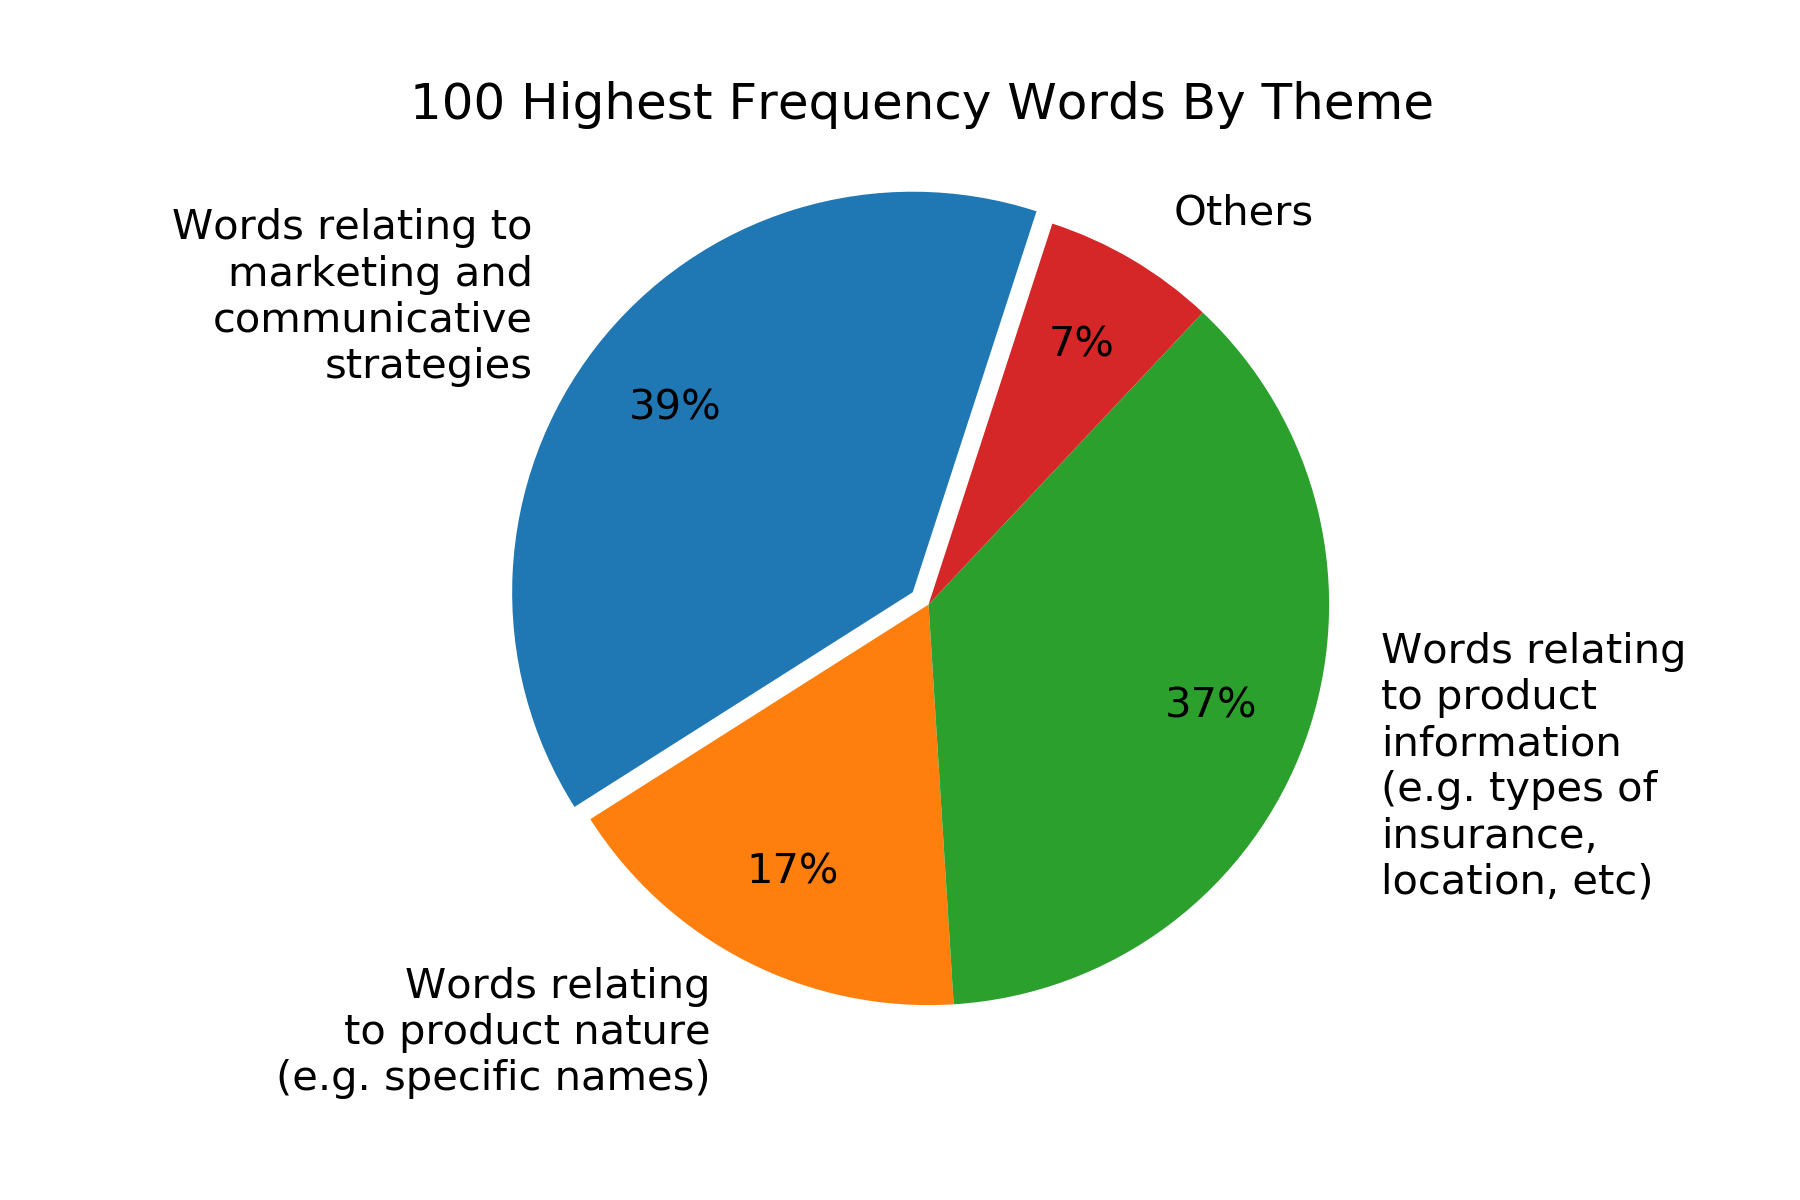
\includegraphics[width=\textwidth]{figures/Figure1.png}
%     \caption{From `Securing Life in Trust: Corpus-based Keyword Analysis of Japanese Insurance TV Commercials' by Svetanant and Ballsun-Stanton. Do not distribute.}
%     \label{fig:userstory}
% \end{figure}

% % \end{column}
% \end{columns}
% \end{frame}
% \begin{frame}{Social Media Research}
% \begin{columns}
% \column{0.5\textwidth}
% \begin{itemize}[label=\textbullet]
%     \item Studying keyword use of local groups.
%     \item Data set from mastodon currently downloading. At 1GB of JSON already. 
%     \item Using Twitter Historical Power Track to run a single massive query for \$2,000
%     \item My first official ``big-data'' (It doesn't run on my laptop)
%     \item Interacting with the raw APIs via python's `requests' module.

% \end{itemize}
% \column{0.5\textwidth}
% \begin{figure}
%     % \centering
%     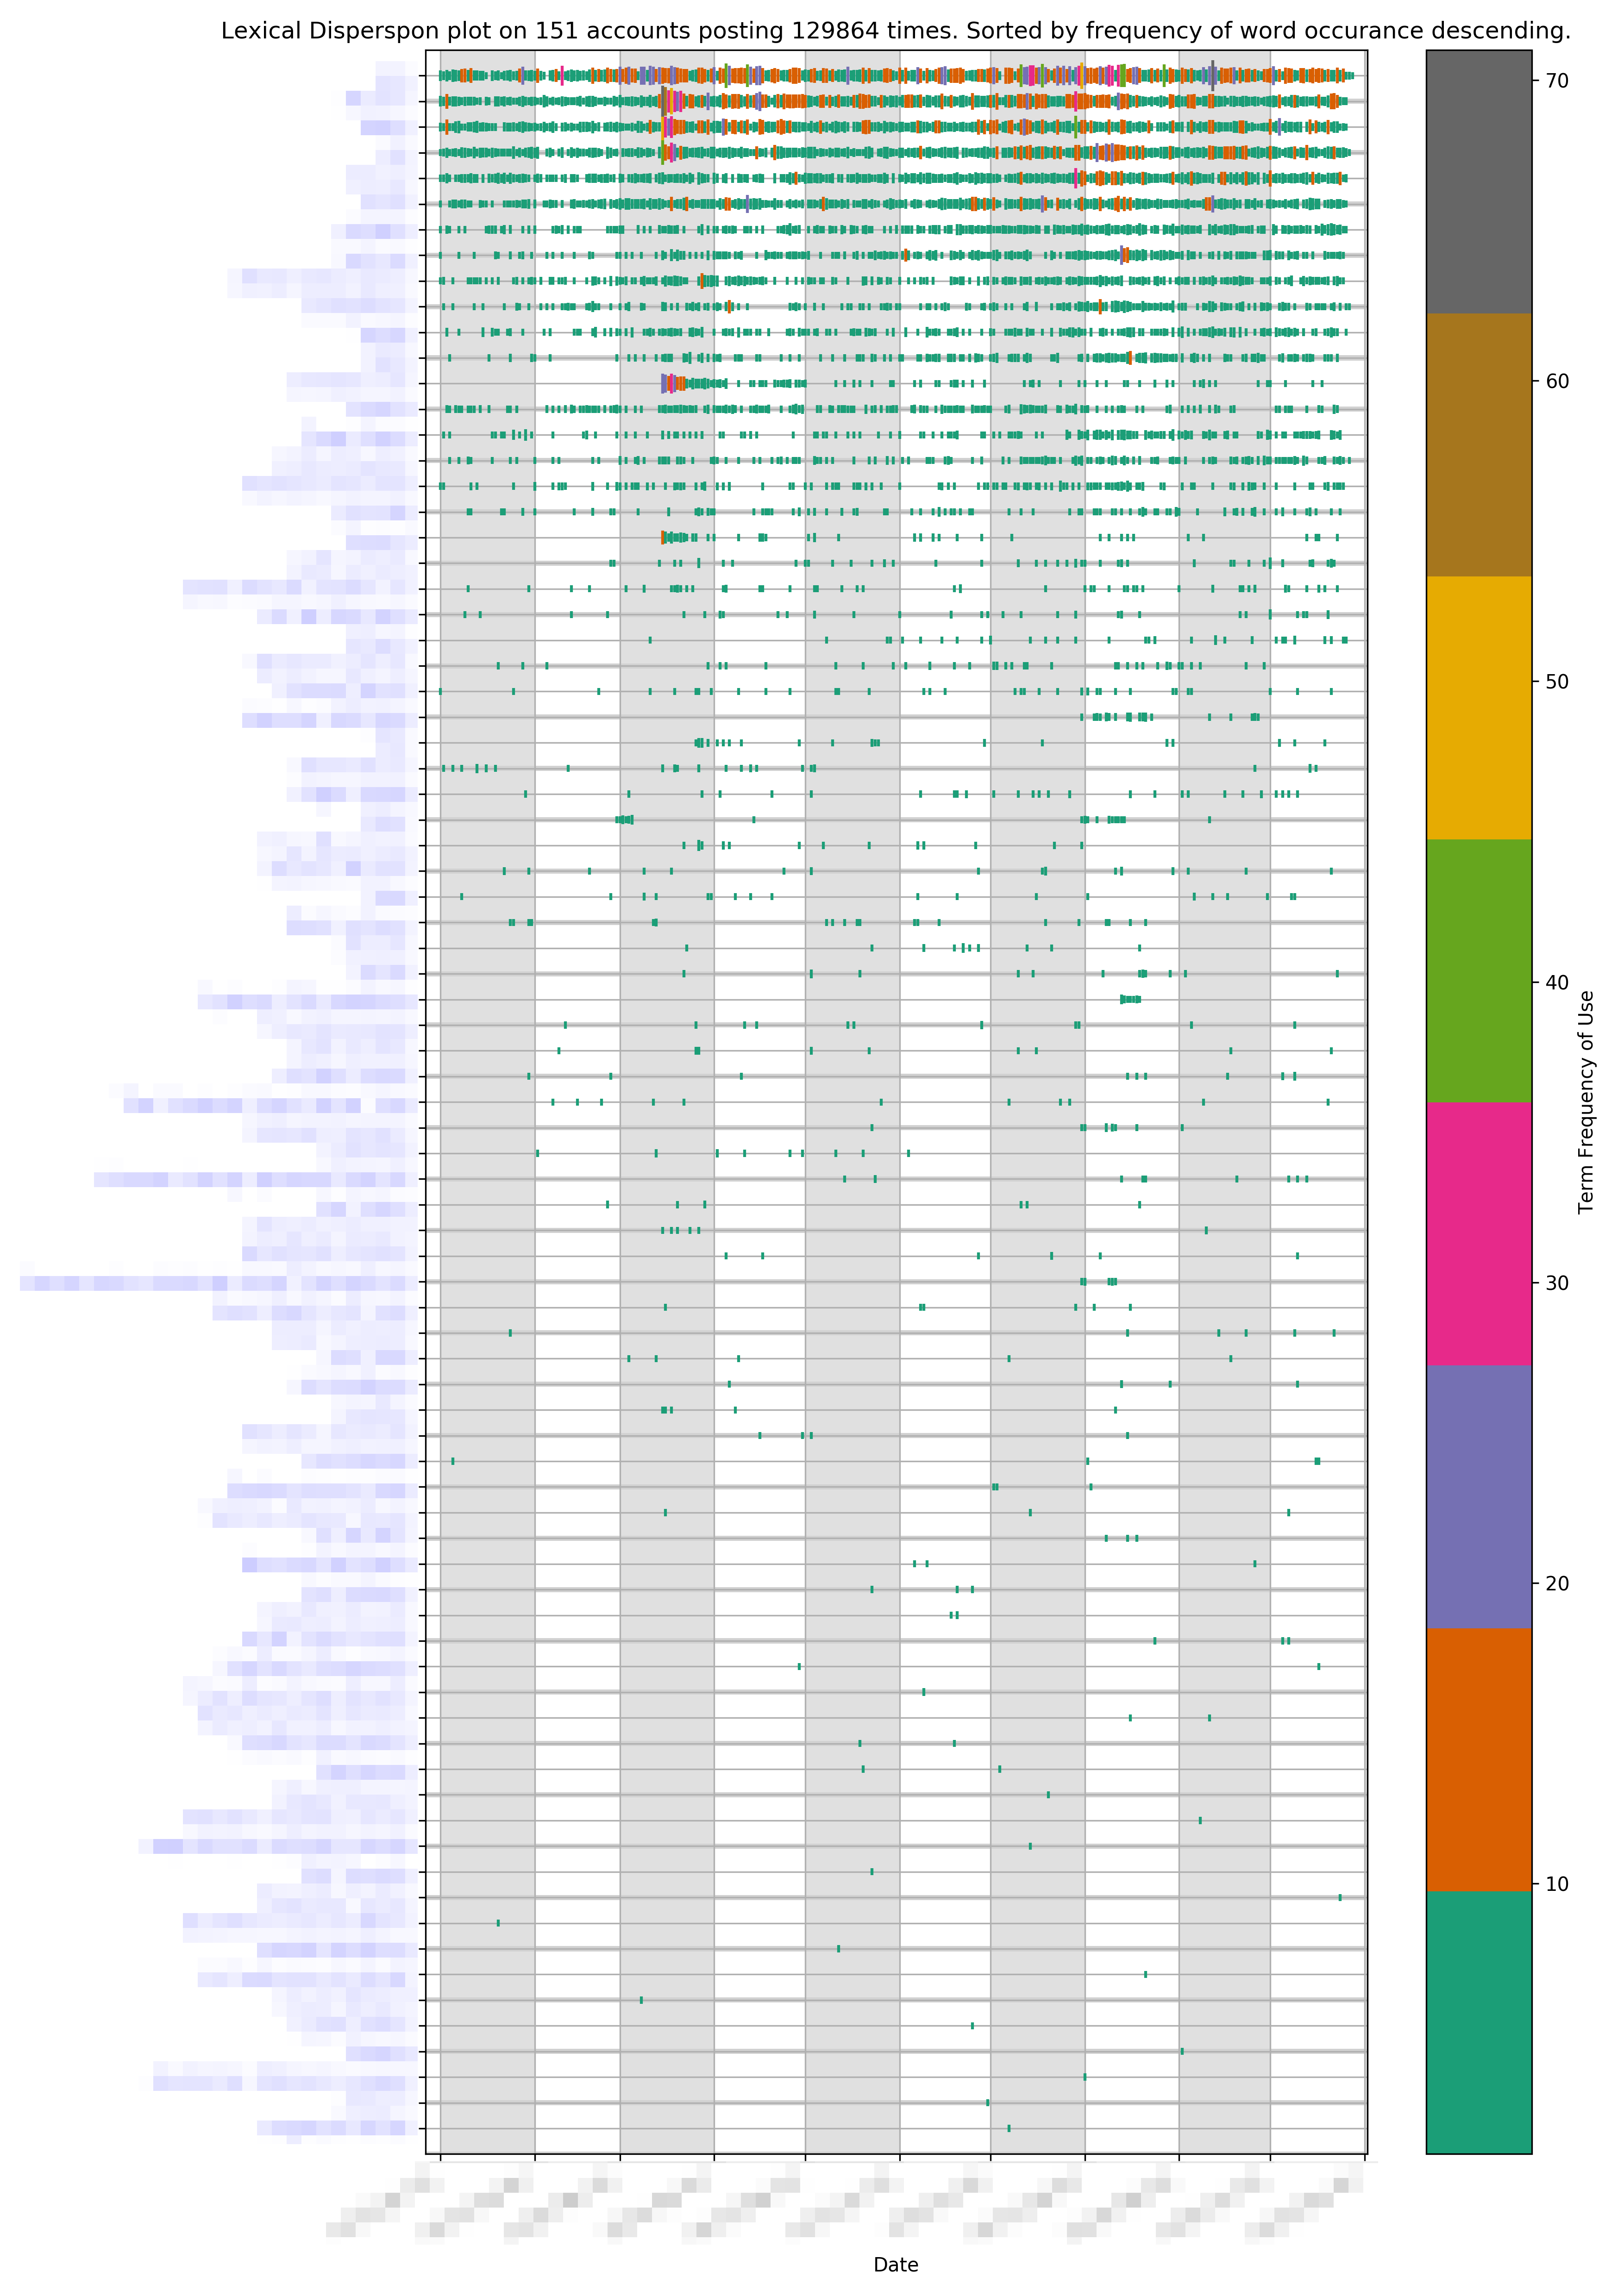
\includegraphics[height=.7\textheight]{figures/blur.png}
%     \caption{Lexical Dispersion plot by Brian Ballsun-Stanton. Blurred due to sensitive ongoing research.}
%     \label{fig:blur}
% \end{figure}
% \end{columns}

% \end{frame}
% \section{Natural Language Processing}

% \begin{frame}{Tools which have produced results}

% \begin{itemize}[label=\textbullet]
% \item Python3
% \item The NLTK book.
% \item MeCAB for Japanese
% \item Log-likelihood computation by Rayson and Garside 2000
% \item Checking dates on stack overflow posts
% \item Filesender
% \item Making sure my code is resume-able
% \item Git
% \item rsub/rmate
% \item byobu
% \end{itemize}
% \end{frame}
% \begin{frame}{Python Modules}

% \begin{itemize}[label=\textbullet]
% \item Using spaCy for tokenisation, lemmatisation. NLTK for stemming.
% \item Matplotlib for a Lexical Dispersion Plot
% \item tqdm
% \item dateparser and Delorean
% \item tldextract
% \item matplotlib 
% \item sqlitedict
% \item wordcloud
% \end{itemize}
% \end{frame}
% \section{Doctesting}
% \begin{frame}{When do I doctest?}
% \begin{columns}
% \column{0.5\textwidth}
% \begin{itemize}
% \item Very slim form of unit testing: 
% \item ``Making sure each function I write does what I want it to do and returns output I want it to return.'' 
% \item Great tool for catching errors introduced when changing a function, especially when it gives data to other functions.
% \item Forces compartmentalisation and documentation of functions.
% \item Really effective in Jupyter Notebooks to test a cell.

% \end{itemize}

% \column{0.5\textwidth}
% \begin{figure}
%     % \centering
%     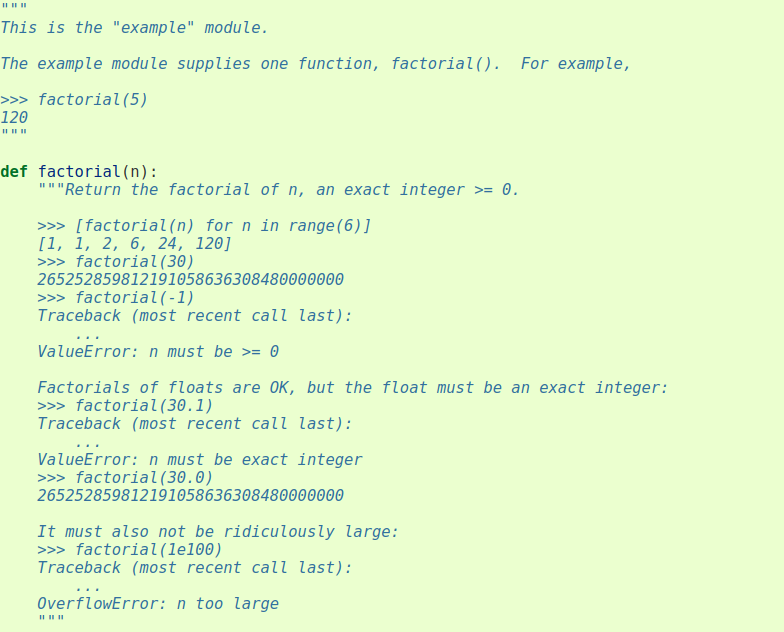
\includegraphics[height=.7\textheight]{figures/screenshotDoctest.png}
%     \caption{From docs.python.org/3.7/library/doctest.html}
%     \label{fig:documentation}
% \end{figure}

% \end{columns}
% \end{frame}
% \begin{frame}{Doctesting in Jupyter}
% \begin{figure}
%     % \centering
%     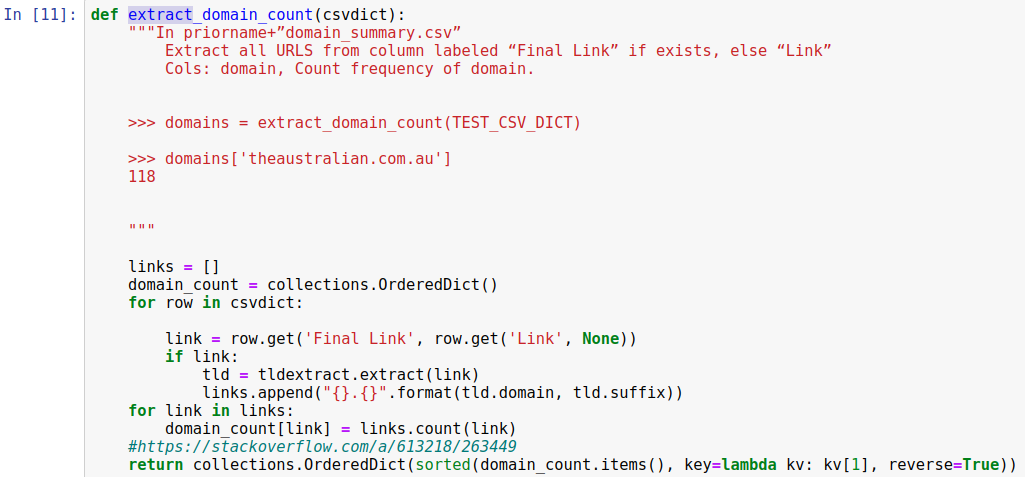
\includegraphics[height=.75\textheight]{figures/jupyterDoctest.png}
%     \caption{From code I wrote to help a Masters student analyise their social media data. GPLv3}
%     \label{fig:analysis}
% \end{figure}
% \end{frame}
% \section{Shell Scripts and Jupyter Notebooks}
% \begin{frame}{Different tools for different purposes}
% \begin{itemize}[label=\textbullet]
%     \item I use Jupyter Notebooks when I'm likely to be sharing the code with researchers.
%     \item See the LIGO black hole mybinder notebook.
%     \item Notebooks are fundamentally narrative and chunked. Tell a story. Encourage Documentation.
%     \item Shell scripts (and python run from the shell) is a "Just run everything." Scales better. Less nonsense, more capable. Run and forget.
% \end{itemize}

% \end{frame}


% \begin{frame}{Thank you!}

% % This presentation is available at:
% % \texttt{https://osf.io/...}

% Source code for this presentation is available at: \url{https://github.com/Denubis/Lessons-learned-from-Data-Analysis-projects}

% This work is licensed under a Creative Commons Attribution 4.0 International License.

% \end{frame}

\section*{References}

\begin{multicols}{2}[]
\bibliography{references}
\bibliographystyle{apalike}
\end{multicols}


% \begin{frame}[allowframebreaks]{References}
  
%   \bibliography{references}
%   \bibliographystyle{apalike}
% \end{frame}


\begin{frame}{Thank you!}

% This presentation is available at:
% \texttt{https://osf.io/...}

Source code for this presentation is available at: \url{https://github.com/MQ-FOAR705/MQ-FOAR705-Week3}

This work is licensed under a Creative Commons Attribution 4.0 International License.

\end{frame}


\end{document}